\documentclass{bioinfo}
\usepackage{booktabs}
\usepackage{amsmath}
\usepackage{amssymb}
\usepackage{bm}
\usepackage{url}
\usepackage[hidelinks]{hyperref}
\setcitestyle{authoryear,round}
\copyrightyear{2026} \pubyear{2026}

\access{Advance Access Publication Date: Day Month Year}
\appnotes{Original Paper}

\begin{document}
\firstpage{1}

\subtitle{Gene expression}

\title[Graph-conditioned state-space models for perturbation prediction]{Graph-conditioned state-space models for
genetic perturbation response prediction: a controlled evaluation against simple baselines}
\author[Padarthi and Huynh]{Aryan Padarthi\,$^{\text{\sfb 1,}*}$ and Riley Huynh\,$^{\text{\sfb 1}}$}
\address{$^{\text{\sfb 1}}$Allen High School, Allen, TX 75013, USA}

\corresp{$^\ast$To whom correspondence should be addressed.}

\history{Received on XXXXX; revised on XXXXX; accepted on XXXXX}

\editor{Associate Editor: XXXXXXX}

\abstract{\textbf{Motivation:} Predicting the transcriptional response to unmeasured genetic
perturbations---in particular to combinations of perturbations---is a central goal of
single-cell perturbation modelling, yet recent benchmarks show that deep models rarely beat
simple additive or linear baselines. State-space models (SSMs) scale linearly with the number of
genes, but genes have no natural order and an SSM has no notion of which genes are related. We
asked whether conditioning an SSM on a gene--gene co-expression graph closes this gap.\\
\textbf{Results:} We introduce GCP-Mamba, a bidirectional selective SSM over all 5,045 measured
genes in which the diffusion of the perturbation over a control-cell co-expression graph modulates
the discretization step of every gene token. On the five standard GEARS splits of the Norman
et al.\ CRISPRa screen, GCP-Mamba gave the lowest error of all methods on unseen single
perturbations, and the true graph outperformed both a label-permuted graph and no graph there.
For double perturbations, however, the additive sum of single-perturbation effects remained
the best predictor, no model explained any of the variance of genetic interactions beyond it, and
graph conditioning of the step size itself had no measurable effect. We also document two
evaluation pitfalls: a perturbation encoding restricted to highly variable genes that silently
discarded 80\% of training perturbations in an earlier version of this work, and a
genetic-interaction correlation metric that scores a predictor of no change close to trained
models.\\
\textbf{Availability and implementation:} Code, splits and all per-condition results are
available at \url{https://github.com/The-MathKing/gcpmamba} (MIT license).\\
\textbf{Contact:} \href{mailto:aryan.padarthi@student.allenisd.org}{aryan.padarthi@student.allenisd.org}\\
\textbf{Supplementary information:} Supplementary data are available at \textit{Bioinformatics}
online.}

\maketitle

% ─────────────────────────────────────────────────────────────────────────────
\section{Introduction}

Perturb-seq screens measure the transcriptome-wide response of single cells to CRISPR-mediated
gene perturbations \citep{dixit2016,norman2019,replogle2022}. Because the number of possible
combinations grows quadratically with the number of targets, only a small fraction of double
perturbations can ever be measured: the Norman et al.\ K562 CRISPRa screen profiled 131 of the
$\binom{105}{2}=5{,}460$ pairs of its 105 targets \citep{norman2019}. Models that predict the
response to unmeasured perturbations---and in particular the non-additive, genetic-interaction
(GI) component of double perturbations---are therefore a central goal of the field.

Knowledge-graph neural networks such as GEARS \citep{roohani2024} and TxPert \citep{wenkel2026},
and transformer-based single-cell foundation models \citep{cui2024scgpt,theodoris2023}, have been
proposed for this task. However, recent benchmarks found that such models often do not outperform
deliberately simple baselines: the mean training response, the sum of single-perturbation effects,
or a low-rank linear model \citep{ahlmann2025,csendes2025}. Two lessons from this literature shape
our study: every new architecture must be compared against these baselines on identical splits, and
the contribution of any biological prior must be isolated by controls that remove it while keeping
everything else fixed.

State-space models (SSMs) such as Mamba \citep{gu2023} process sequences in time and memory linear
in their length, whereas self-attention is quadratic \citep{vaswani2017}. Treating the transcriptome
as a sequence of gene tokens, an SSM can process all measured genes at once, but genes have no
natural order and the recurrence has no notion of which genes are functionally related. We asked
whether both limitations can be addressed by conditioning the SSM's discretization step on a
gene--gene graph, and---more importantly---whether doing so yields better predictions than simple
baselines.

Our contributions are: (i) GCP-Mamba, a bidirectional selective SSM over all measured genes in which
the diffusion of the perturbation over a co-expression graph modulates the step size of every gene
token; (ii) a controlled benchmark on the five standard GEARS splits of the Norman data and on the
Adamson et al.\ CRISPRi screen, against five simple baselines, GEARS retrained on the same splits,
and eight ablations and variants that remove, permute or relocate the graph, destroy the gene
ordering, remove the recurrence or add an additive prior; and (iii) two evaluation pitfalls, one of
which invalidated the conclusions of an earlier version of this work.

% ─────────────────────────────────────────────────────────────────────────────
\section{Methods}

\subsection{Data and splits}
We used the Norman et al.\ K562 CRISPRa Perturb-seq data \citep{norman2019} as distributed with
GEARS: 91{,}205 cells, 5{,}045 genes, 7{,}353 control cells, single perturbations of 105 genes and
131 double perturbations, log-normalised. For every condition $p$ we computed the pseudobulk
response $\bm{\delta}_p=\bar{\mathbf{x}}_p-\bar{\mathbf{x}}_{\mathrm{ctrl}}\in\mathbb{R}^{5045}$.
Singles are recorded as two conditions (\texttt{A+ctrl}, \texttt{ctrl+A}) that use different guides;
wherever a single response is needed we average them. We used the GEARS \emph{simulation} splits
with seeds 1--5, generated with the official \texttt{cell-gears} code \citep{roohani2024}. Each holds
out about a quarter of the targets; test perturbations are grouped into unseen singles and doubles
with zero, one or two targets seen during training (``0/2'', ``1/2'', ``2/2 seen''; GEARS counts a
target as seen if it appears in the training or validation set). Across the five splits the test
sets contain 185 unseen-single, 32 ``0/2'', 254 ``1/2'' and 90 ``2/2'' perturbations.
Validation perturbations were used only for early stopping and for choosing the ridge penalty of
the linear baselines. As a second dataset we used the Adamson et al.\ K562 CRISPRi screen
\citep{adamson2016} (86 single perturbations, 5{,}060 genes; GEARS simulation splits, seeds 1--5).

The co-expression graph, gene embeddings and gene order below were computed from unperturbed
control cells only; they are identical in every split and contain no information about any
perturbation response.

\subsection{Co-expression graph and perturbation signal}
We z-scored control-cell expression, computed absolute Pearson correlations between all gene
pairs, kept the $k=20$ strongest neighbours of every gene and symmetrised the result, giving a
sparse graph $\mathbf{W}$ with 111{,}078 edges. For a perturbation set $P$ with indicator
$\mathbf{1}_P\in\{0,1\}^G$, the graph signal is a truncated diffusion
\begin{equation}
\mathbf{c}(P)=\log\!\Big(1+s\sum_{k=1}^{3}\beta^{k-1}\,\widetilde{\mathbf{W}}^{k}\mathbf{1}_P\Big),
\qquad \widetilde{\mathbf{W}}=\mathbf{D}^{-1/2}\mathbf{W}\mathbf{D}^{-1/2},
\end{equation}
with degree matrix $\mathbf{D}$, $\beta=0.5$ and $s=10^{3}$ (the logarithm compresses values that
span four orders of magnitude). $c_i(P)$ is large for genes close to a perturbed gene in the graph
and zero for genes more than three steps away.

\subsection{GCP-Mamba}
\label{sec:model}
The model is summarised in Figure~\ref{fig:arch}.

\textbf{Tokens.} Each of the $G$ genes is one token. Token $i$ is the sum of a learned identity
vector, a projection of the gene's control-cell embedding $\mathbf{e}_i$ (its loadings on the top
64 principal components of control-cell expression, standardised) and of its control mean
expression. A perturbation enters in three ways: (i) a learned flag vector added to the tokens of the
targeted genes; all targets are measured genes, so no perturbation is lost (Section~\ref{sec:pitfall});
(ii) a set embedding $\mathbf{z}_P=\sum_{g\in P}\big(f(\mathbf{e}_g)+\mathbf{t}_g\big)$ added to every
token, where $f$ is a two-layer MLP and $\mathbf{t}_g$ a per-target vector initialised at zero; only
targets perturbed in training receive gradient for $\mathbf{t}_g$, so a target never seen in
training is represented through $f(\mathbf{e}_g)$ alone, which is what permits zero-shot prediction;
and (iii) the graph signal $c_i(P)$, linearly projected and added to token $i$.

\textbf{Graph-conditioned selective scan.} Each of two layers applies a forward and a backward
Mamba-style selective SSM \citep{gu2023} with diagonal state matrix
$\mathbf{A}=-\mathrm{diag}(1,\dots,N)$, input-dependent $\mathbf{B}_i$ and $\mathbf{C}_i$, a SiLU
output gate and a skip connection. The step size is conditioned on the graph,
\begin{equation}
\bm{\Delta}_i=\mathrm{softplus}\big(\mathbf{W}_{\Delta}\mathbf{u}_i+\mathbf{b}_{\Delta}+\mathbf{w}_c\,c_i(P)\big),
\end{equation}
where $\mathbf{u}_i$ is the layer input and $\mathbf{w}_c\in\mathbb{R}^{d}$ is learned and
initialised at zero, so that the model starts as an unconditioned SSM. With zero-order-hold
discretization, $\mathbf{h}_i=\exp(\bm{\Delta}_i\mathbf{A})\,\mathbf{h}_{i-1}+\bm{\Delta}_i\mathbf{B}_i u_i$:
tokens near the perturbation take larger steps, writing more of their input into the state and
forgetting more of the past. Because $\mathbf{w}_c c_i(P)$ differs between genes and between
perturbations, permuting the graph changes the function the model computes.

\textbf{Gene order.} Genes are placed along the Fiedler vector \citep{fiedler1973} of the normalised
Laplacian of $\mathbf{W}$, so that strongly co-expressed genes are close in the sequence.

\textbf{Readout.} The prediction for gene $i$ is
$\hat\delta_i=b_i+\mathbf{w}^{\top}\mathbf{h}_i+(\mathbf{U}\mathbf{h}_i)^{\top}(\mathbf{V}\mathbf{z}_P)$,
where $\mathbf{h}_i$ is the final token state and $\mathbf{U},\mathbf{V}$ have rank 16. The bilinear
term expresses a gene-by-perturbation interaction and contains the low-rank linear model of
\citet{ahlmann2025} as a special case. The bias $b_i$ is initialised at the mean training response
and $\mathbf{w}$ and $\mathbf{V}$ at zero, so that training starts from the \emph{train-mean}
baseline and learns deviations from it; without this initialisation, and without standardising
$\mathbf{e}_g$, the model did not improve on the train-mean baseline in pilot runs on the
validation set of split 1 (Supplementary Section~S2).

\textbf{Implementation and complexity.} We implemented the scan in PyTorch as an exact chunked
parallel scan: cumulative sums in log space within chunks of 16 tokens and a sequential recurrence
across chunk states. Per-step log-decays are clamped at $-5$ (a decay factor of at least 0.0067) so
that the within-chunk exponentials remain finite in single precision; the implementation matches a
naive sequential recurrence to $10^{-5}$ (unit test in the repository). Time and memory are
$\mathcal{O}(BGdN)$ for the scan and $\mathcal{O}(|\mathbf{W}|)$ for the sparse diffusion, i.e.\
linear in the number of genes; no $G\times G$ object is formed.

\textbf{Training.} $d=32$, $N=4$, dropout 0.1 in $f$; AdamW \citep{loshchilov2019} with learning
rate $10^{-3}$, weight decay $10^{-2}$ and batch size 8; gradient clipping at 1; mean-squared error
over all genes. Models were trained for at least 40 and at most 100 epochs and stopped 15 epochs
after the last improvement of the validation loss; the state with the lowest validation loss was
kept. (The validation loss typically plateaus for several epochs before a model starts to use the
perturbation; without the 40-epoch minimum, patience-based stopping truncated some runs during
this plateau.) The model seed equals the split seed. All runs used a 4-core CPU; one training run
took 5--25 minutes.

\subsection{Ablations and variants}
All variants share the architecture, perturbation inputs (i)--(ii), optimiser and stopping rule, and
differ in one factor. \emph{$\Delta$ only}: the graph enters only through $\bm\Delta$, not through the
tokens. \emph{$\Delta$ only, $\mathbf{w}_c\sim\mathcal{N}(0,1)$}: as before, but $\mathbf{w}_c$ is
initialised randomly so that the conditioning is active from the start. \emph{Permuted graph}: the gene
labels of $\mathbf{W}$ are randomly permuted, which preserves its degree distribution and spectrum.
\emph{Random order}: genes are placed in random order instead of the Fiedler order. \emph{Mamba (no
graph)}: $c(P)\equiv0$. \emph{Graph-MLP}: the SSM layers are replaced by per-token MLPs, so genes
interact only through $\mathbf{z}_P$ and the graph signal. \emph{Additive prior}: the network predicts
the residual $\bm{\delta}-\bm{\pi}$ with respect to the additive prior $\bm{\pi}$ (the sum of the
targets' observed single responses, or the mean single response for an unseen target; for single
perturbations always the mean single response), with and without the graph.

\subsection{Baselines}
\emph{No change} predicts $\bm{\delta}=\mathbf{0}$. \emph{Train mean} predicts the mean training
response. \emph{Additive} predicts the sum of the targets' single responses observed during training
(training or validation set), substituting the mean single response for a target without one.
\emph{Linear} is the model of \citet{ahlmann2025},
$\mathbf{Y}\approx\mathbf{G}\mathbf{M}\mathbf{P}^{\top}+\mathbf{b}$, with gene embeddings $\mathbf{G}$
from the top 10 principal components of the training responses and each perturbation represented by
the sum of its targets' embeddings, taken either from $\mathbf{G}$ (\emph{Linear (PCA)}, as in the
original) or from the control-cell embeddings $\mathbf{e}_g$ that GCP-Mamba receives
(\emph{Linear (ctrl emb.)}); the ridge penalty was chosen on the validation set from
$\{10^{-3},\dots,10^{4}\}$. \emph{GEARS} was retrained with the official implementation and default
hyperparameters (hidden size 64, 20 epochs) on the same splits.

\subsection{Metrics and statistics}
Following \citet{roohani2024}, for every test perturbation we computed the mean squared error (MSE)
and the Pearson correlation between predicted and observed $\bm\delta$ on its top-20 differentially
expressed (DE) genes. For double perturbations $AB$ we computed the GI residual
$\bm{\epsilon}=\bm{\delta}_{AB}-\bm{\delta}_{A}-\bm{\delta}_{B}$ from the measured singles (used only
for scoring). The MSE of a predicted residual $\hat{\bm\delta}_{AB}-\bm{\delta}_{A}-\bm{\delta}_{B}$
equals the MSE of $\hat{\bm\delta}_{AB}$ itself, so it carries no extra information. We therefore
report the fraction of GI variance explained,
$R^2_{\mathrm{GI}}=1-\sum_{AB}\mathrm{MSE}_{AB}\big/\sum_{AB}\overline{\epsilon^2_{AB}}$, on ``2/2
seen'' doubles, where the additive baseline is exactly the measured-singles sum and scores 0, and the
Pearson correlation between predicted and observed residuals used in earlier work. Metrics were
averaged over the test perturbations of a split and are reported as mean\,$\pm$\,s.d.\ over the
five splits. We compared GCP-Mamba with every other model using two-sided Wilcoxon signed-rank tests
on per-perturbation differences pooled across splits, with Holm correction within each
metric and test group (Supplementary Table~S3). Because perturbations recur across splits these
pooled tests are approximate, and we emphasise effect sizes and their consistency across splits.

% ─────────────────────────────────────────────────────────────────────────────
\begin{figure*}[!t]
\centerline{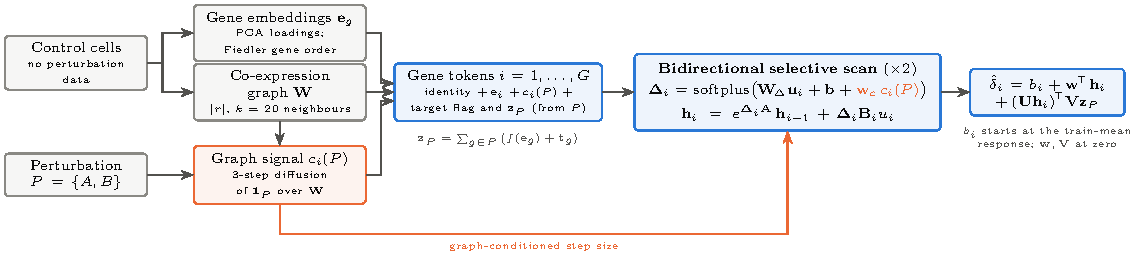
\includegraphics[width=\textwidth]{fig_arch.pdf}}
\caption{GCP-Mamba. Everything derived from expression (grey) is computed from control cells only.
The perturbation enters the gene tokens (a target flag and the set embedding $\mathbf{z}_P$) and,
through its diffusion $c_i(P)$ over the co-expression graph (orange), the step size $\bm\Delta_i$ of
every token in the bidirectional selective scan. The bilinear readout starts at the train-mean
prediction.}\label{fig:arch}
\end{figure*}

\section{Results}

\subsection{A perturbation encoding restricted to highly variable genes discards most perturbations}
\label{sec:pitfall}
An earlier version of this study encoded a perturbation as a multi-hot vector over the 500 most
highly variable genes (HVGs), the same genes whose expression was predicted, and parsed single
perturbations from the condition name with a rule that mapped \texttt{ctrl+A} to the control
condition. Only 12--17 of the 105 CRISPRa targets were among the HVGs (mean 14 over the ten
splits used then), so 77--84\% of training perturbations (mean 80\%) and 70--94\% of test
perturbations received an all-zero input, and the 161--183 training perturbations of a split shared
only 14--19 distinct input vectors (Supplementary Table~S1; \texttt{gcpm/audit\_hvg\_encoding.py}).
A model cannot distinguish perturbations it receives as identical inputs, so that version could at
best learn the mean response; its negative conclusion about graph conditioning was an artefact of
the encoding, not a property of the architecture. The problem is easy to miss: training converges,
loss curves look normal, and the model is competitive with the train-mean baseline. It applies to any
model whose perturbation input is indexed by the output gene set. Here every target is represented
by its own token and by an embedding computed from control cells, and we recommend that
perturbation models report how many targets reach the input.

\subsection{Unseen single perturbations benefit from the graph; double perturbations do not}

Table~\ref{tab:main} and Figure~\ref{fig:bench} compare GCP-Mamba with the baselines and GEARS on
the Norman data. As in previous benchmarks \citep{ahlmann2025}, the additive baseline was the most
accurate predictor overall (MSE 0.240 on the top-20 DE genes, averaged over all test perturbations) %NUM
and for doubles with at least one seen target; for ``2/2 seen'' doubles its error (0.089) was half %NUM
that of any trained model. GCP-Mamba (0.278) improved substantially on the train-mean (0.428), %NUM
linear (0.349) and no-change (0.561) baselines, and on GEARS (TBD). %NUM

For unseen single perturbations, where no additive information exists, GCP-Mamba had the lowest
error of all methods (0.255 vs.\ 0.270 for the train mean, 0.269 for the linear model and TBD for %NUM
GEARS; Holm-adjusted $P=0.039$ vs.\ train mean and $P=0.24$ vs.\ the linear model). On the same %NUM
perturbations the true co-expression graph outperformed a label-permuted graph (0.257; $P=0.017$) %NUM
and no graph (0.266; $P=0.014$), so the gain on unseen singles depends on the content of the graph %NUM
and not only on its presence. The effects are small, however: the median per-perturbation
improvement over the train mean was 0.003 (1--2\% of the error), smaller than the variation %NUM
between splits (Fig.~\ref{fig:bench}). For doubles with only one seen target (``1/2 seen'') the
recurrent models were far behind the additive baseline (0.309 vs.\ 0.239) and adding the graph to %NUM
the tokens increased the error relative to no graph (0.309 vs.\ 0.292; $P=0.019$). %NUM

\begin{figure*}[!t]
\centerline{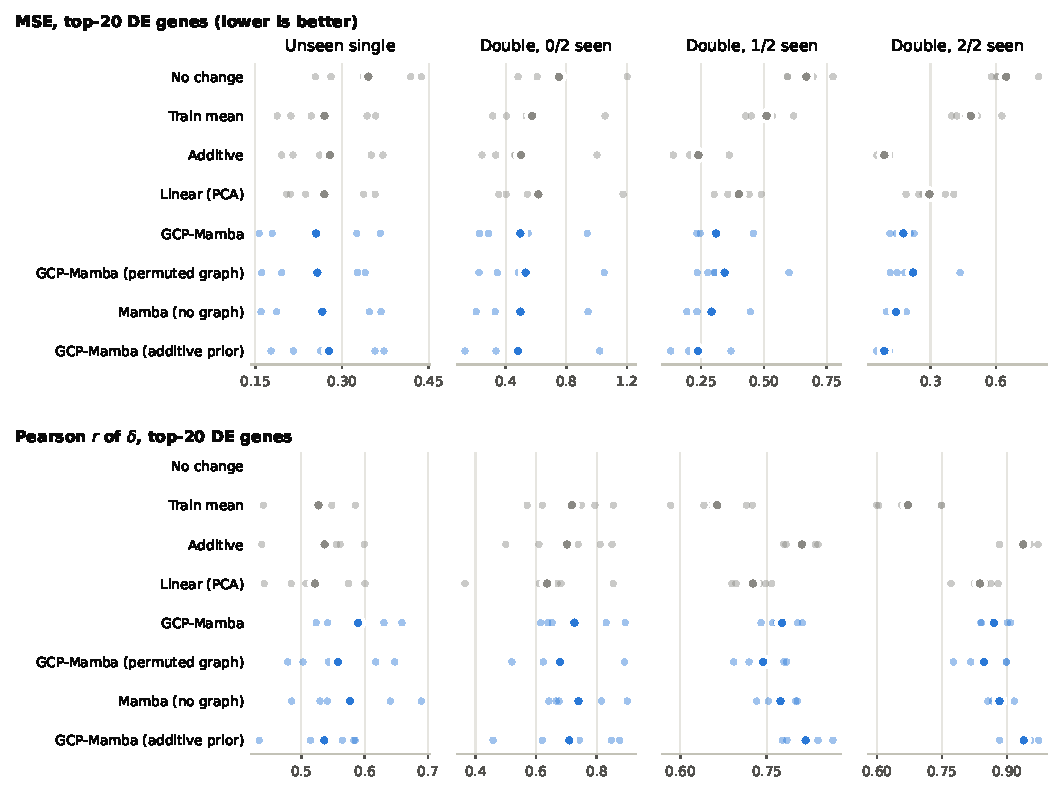
\includegraphics[width=\textwidth]{fig_benchmark.pdf}}
\caption{Norman et al.\ CRISPRa data, five GEARS simulation splits. Each large dot is the mean over
splits and each small dot one split; columns are test groups. Top: MSE on the top-20 DE genes of each
test perturbation (lower is better). Bottom: Pearson correlation of predicted and observed change on
the same genes (undefined for \emph{No change}). Grey, baselines; orange, GEARS; blue, GCP-Mamba and
variants.}\label{fig:bench}
\end{figure*}

\begin{table*}[!t]
\processtable{Norman et al.\ CRISPRa screen: MSE of the predicted expression change on the top-20 DE genes of each test perturbation (mean\,$\pm$\,s.d.\ over the five GEARS simulation splits; lower is better; best in bold)\label{tab:main}}{
\begin{tabular*}{\hsize}{@{\extracolsep{\fill}}lccccc@{}}
\toprule
Model & Unseen single & Double, 0/2 seen & Double, 1/2 seen & Double, 2/2 seen & All test \\
\midrule
No change & 0.346\,$\pm$\,0.081 & 0.752\,$\pm$\,0.272 & 0.669\,$\pm$\,0.077 & 0.647\,$\pm$\,0.087 & 0.561\,$\pm$\,0.061 \\
Train mean & 0.270\,$\pm$\,0.077 & 0.576\,$\pm$\,0.287 & 0.511\,$\pm$\,0.076 & 0.485\,$\pm$\,0.092 & 0.428\,$\pm$\,0.061 \\
Additive & 0.279\,$\pm$\,0.079 & 0.501\,$\pm$\,0.295 & \textbf{0.239\,$\pm$\,0.081} & \textbf{0.089\,$\pm$\,0.022} & \textbf{0.240\,$\pm$\,0.070} \\
Linear (PCA) & 0.269\,$\pm$\,0.073 & 0.616\,$\pm$\,0.328 & 0.400\,$\pm$\,0.073 & 0.296\,$\pm$\,0.090 & 0.349\,$\pm$\,0.059 \\
Linear (ctrl emb.) & 0.322\,$\pm$\,0.103 & 0.962\,$\pm$\,0.788 & 0.518\,$\pm$\,0.090 & 0.413\,$\pm$\,0.122 & 0.452\,$\pm$\,0.078 \\
\midrule
GCP-Mamba & \textbf{0.255\,$\pm$\,0.091} & \textbf{0.497\,$\pm$\,0.280} & 0.309\,$\pm$\,0.090 & 0.176\,$\pm$\,0.046 & 0.278\,$\pm$\,0.079 \\
\botrule
\end{tabular*}}{}
\end{table*}

\begin{table*}[!t]
\processtable{Ablations and residual variants on the Norman data: MSE on the top-20 DE genes (mean\,$\pm$\,s.d.\ over five splits; best in bold)\label{tab:ablation}}{
\begin{tabular*}{\hsize}{@{\extracolsep{\fill}}lccccc@{}}
\toprule
Model & Unseen single & Double, 0/2 seen & Double, 1/2 seen & Double, 2/2 seen & All test \\
\midrule
GCP-Mamba & \textbf{0.255\,$\pm$\,0.091} & 0.497\,$\pm$\,0.280 & 0.309\,$\pm$\,0.090 & 0.176\,$\pm$\,0.046 & 0.278\,$\pm$\,0.079 \\
\midrule
GCP-Mamba ($\Delta$ only) & 0.260\,$\pm$\,0.086 & 0.503\,$\pm$\,0.297 & 0.300\,$\pm$\,0.116 & 0.158\,$\pm$\,0.064 & 0.274\,$\pm$\,0.095 \\
GCP-Mamba ($\Delta$ only, $\mathbf{w}_c\sim\mathcal{N}(0,1)$) & 0.266\,$\pm$\,0.091 & 0.492\,$\pm$\,0.296 & 0.304\,$\pm$\,0.088 & 0.154\,$\pm$\,0.024 & 0.276\,$\pm$\,0.081 \\
GCP-Mamba (permuted graph) & 0.257\,$\pm$\,0.079 & 0.531\,$\pm$\,0.317 & 0.344\,$\pm$\,0.146 & 0.221\,$\pm$\,0.126 & 0.304\,$\pm$\,0.115 \\
GCP-Mamba (random order) & 0.263\,$\pm$\,0.078 & 0.526\,$\pm$\,0.232 & 0.303\,$\pm$\,0.092 & 0.158\,$\pm$\,0.053 & 0.276\,$\pm$\,0.075 \\
Mamba (no graph) & 0.266\,$\pm$\,0.093 & 0.498\,$\pm$\,0.279 & 0.292\,$\pm$\,0.096 & 0.142\,$\pm$\,0.034 & 0.269\,$\pm$\,0.086 \\
Graph-MLP (no scan) & 0.258\,$\pm$\,0.080 & 0.526\,$\pm$\,0.290 & 0.323\,$\pm$\,0.110 & 0.203\,$\pm$\,0.082 & 0.291\,$\pm$\,0.089 \\
\midrule
GCP-Mamba (additive prior) & 0.277\,$\pm$\,0.086 & \textbf{0.482\,$\pm$\,0.330} & \textbf{0.237\,$\pm$\,0.087} & 0.089\,$\pm$\,0.022 & \textbf{0.238\,$\pm$\,0.077} \\
Mamba (additive prior) & 0.279\,$\pm$\,0.085 & 0.491\,$\pm$\,0.328 & 0.237\,$\pm$\,0.088 & \textbf{0.089\,$\pm$\,0.022} & 0.239\,$\pm$\,0.076 \\
\botrule
\end{tabular*}}{}
\end{table*}

\begin{table}[!t]
\processtable{Prediction of genetic interactions (GI) in double perturbations (top-20 DE genes; mean\,$\pm$\,s.d.\ over five splits). $R^2_{\mathrm{GI}}$ is the fraction of the variance of the GI residual $\boldsymbol{\epsilon}$ that a prediction explains; an exactly additive prediction scores 0. The GI Pearson $r$ gives the trivial \emph{No change} and \emph{Train mean} predictors scores close to those of the deep models.\label{tab:gi}}{
\begin{tabular*}{\columnwidth}{@{\extracolsep{\fill}}lcc@{}}
\toprule
Model & $R^2_{\mathrm{GI}}$ $\uparrow$ & GI Pearson $r$ $\uparrow$ \\
\midrule
No change & -11.79\,$\pm$\,1.28 & 0.23\,$\pm$\,0.12 \\
Train mean & -8.53\,$\pm$\,1.11 & 0.26\,$\pm$\,0.12 \\
Additive & -0.76\,$\pm$\,0.45 & 0.26\,$\pm$\,0.12 \\
Linear (PCA) & -4.79\,$\pm$\,1.47 & 0.27\,$\pm$\,0.14 \\
Linear (ctrl emb.) & -7.03\,$\pm$\,1.66 & 0.27\,$\pm$\,0.11 \\
GCP-Mamba & -2.53\,$\pm$\,1.09 & 0.35\,$\pm$\,0.09 \\
Mamba (no graph) & -1.79\,$\pm$\,0.46 & 0.39\,$\pm$\,0.05 \\
GCP-Mamba (additive prior) & -0.77\,$\pm$\,0.46 & 0.30\,$\pm$\,0.07 \\
Mamba (additive prior) & -0.76\,$\pm$\,0.46 & 0.27\,$\pm$\,0.11 \\
\botrule
\end{tabular*}}{}
\end{table}


\subsection{Graph conditioning of the step size has no measurable effect}
Table~\ref{tab:ablation} isolates the components of GCP-Mamba. Conditioning the step size alone
($\Delta$ only) gave results indistinguishable from a plain bidirectional Mamba without the graph %NUM
(0.274 vs.\ 0.269 overall), and the learned conditioning weights stayed close to their zero %NUM
initialisation ($\|\mathbf{w}_c\|=0.07$ per SSM, against 0.56 when the graph is also added to the %NUM
tokens). This was not merely a failure to move away from zero: initialising $\mathbf{w}_c$ randomly, %NUM
so that the step size depends strongly on graph proximity from the first update
($\|\mathbf{w}_c\|\approx5.8$ after training), again changed the error only marginally (0.276). %NUM
Graph proximity to the perturbation thus had little influence on how the SSM propagates information,
whichever way the conditioning was initialised. What distinguished the models was instead the
recurrence: replacing the scan with per-gene MLPs increased the error (0.291 vs.\ 0.278; %NUM
$P=4\times10^{-4}$), while the Fiedler ordering was not better than a random order (0.276). %NUM

\subsection{No model predicts genetic interactions beyond the additive baseline}
Double perturbations are interesting chiefly for their non-additive component. Letting the network
predict the residual with respect to the additive prior closed the gap to the additive baseline
overall (0.238 vs.\ 0.240) but did not improve on it (Table~\ref{tab:ablation}), and on ``2/2 seen'' %NUM
doubles no trained model explained any of the GI variance: $R^2_{\mathrm{GI}}$ was essentially zero
for the residual models (i.e.\ they learned a negligible correction to the additive prior) and
strongly negative for all others (Table~\ref{tab:gi}).

The GI Pearson correlation, used to assess GI prediction in earlier work including the first version
of this study, told a different story (Fig.~\ref{fig:gi}). It rated the recurrent models above the
additive baseline, and it gave the trivial no-change and train-mean predictors values (0.23 and 0.26) %NUM
comparable to the additive baseline and the linear model. This happens because predicting no change
yields a predicted residual of $-(\bm\delta_A+\bm\delta_B)$, which is correlated with the true
residual whenever the interaction is buffering (sub-additive), as it often is. A correlation between
residuals therefore rewards shrinkage towards zero and should not be used alone to claim GI
prediction; a variance-explained measure relative to the additive prediction avoids this.

\begin{figure}[!t]
\centerline{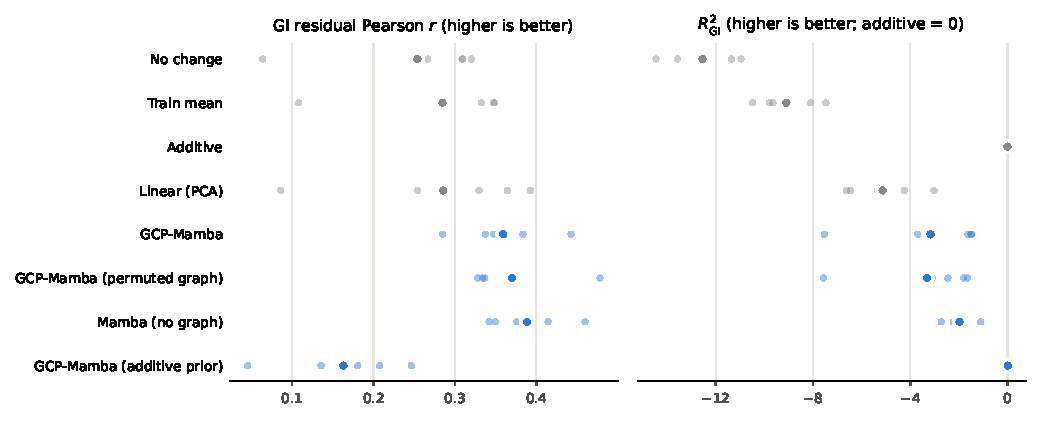
\includegraphics[width=\columnwidth]{fig_gi.pdf}}
\caption{Genetic-interaction prediction on ``2/2 seen'' doubles of the Norman data. Left: Pearson
correlation between predicted and observed GI residuals, which rates trivial predictors close to
trained models. Right: fraction of GI variance explained ($R^2_{\mathrm{GI}}$; the additive baseline
is 0 by construction). Dots as in Fig.~\ref{fig:bench}.}\label{fig:gi}
\end{figure}

\subsection{Adamson CRISPRi screen}
On the Adamson data, which contain only single perturbations, TBD (Table~\ref{tab:adamson}). %NUM

\subsection{Computational cost}
Figure~\ref{fig:scaling} reports the measured time and peak memory of one training step as a function
of the number of gene tokens. TBD %NUM

% ─────────────────────────────────────────────────────────────────────────────
\section{Discussion}

We set out to test whether conditioning a linear-time state-space model on a gene--gene graph yields
better predictions of perturbation responses than simple baselines. With inputs that represent every
perturbation, a training procedure that starts from the train-mean prediction, and controls that
isolate each component, the answer is mixed. The graph helped where the model has least to go on---
single perturbations of genes never perturbed in training---and a permuted graph did not, so the model
does extract information from co-expression neighbourhoods. The improvement was, however, small and
comparable to the variation between splits. For double perturbations, the sum of single effects
remained the best predictor, consistent with \citet{ahlmann2025}, and none of our models, nor GEARS,
explained any of the variance of genetic interactions beyond it.

The mechanism that motivated the architecture---modulating the SSM step size by graph proximity---had
no measurable effect in any of our experiments, whether the conditioning weights started at zero or
at random values. The benefit on unseen singles came from supplying the graph signal as a token
feature, which a non-recurrent model can also exploit. We see two reasons. First, a step-size change
alters how quickly the state forgets, but with a bidirectional scan over 5,045 tokens and short
effective memory, most of the information a token needs is already available locally or through the
shared perturbation embedding. Second, the Norman responses are dominated by a few programs (e.g.\
erythroid and granulocyte differentiation in K562), so a low-rank readout captures most of the
explainable variance, leaving little that a gene-specific propagation mechanism could add.

Our results carry three practical lessons. (i) The input encoding must be audited: an encoding tied
to the output gene set discarded most perturbations in an earlier version of this work without any
visible symptom in training. (ii) Deep models for this task should be initialised at, or explicitly
compared with, the train-mean and additive predictors; without that initialisation our model did not
improve on the train mean at all. (iii) Genetic-interaction prediction should be measured as variance
explained relative to the additive prediction on doubles whose singles were observed; correlations
between residuals reward shrinkage.

\textbf{Limitations.} We evaluated two K562 screens with the standard GEARS splits; screens in other
cell types, genome-wide single-perturbation screens and larger combinatorial libraries may behave
differently, and the Replogle et al.\ screens could not be included because most of their targets are
not among the measured genes in the GEARS release, which our token-based encoding requires. Each
split was trained with one seed, so between-split variation includes model-initialisation variation.
Hyperparameters were chosen on the validation set of the first split only, and not tuned per variant.
We used a single co-expression graph from control cells; knowledge graphs such as Gene Ontology or
protein interaction networks \citep{roohani2024,wenkel2026} might carry complementary information.
Finally, our PyTorch scan runs on CPU; a fused GPU kernel would change absolute run times but not
the linear scaling.

\section*{Acknowledgements}
We thank the authors of GEARS for releasing their code and processed data.

\section*{Author contributions}
A.P.\ designed the model and performed the computational experiments; R.H.\ contributed to the
biological interpretation and to writing. Both authors approved the final manuscript.

\section*{Funding}
This work received no specific funding.

\medskip
\noindent\textit{Conflict of interest:} none declared.

\section*{Data availability}
The Norman et al.\ and Adamson et al.\ data are available from NCBI GEO (GSE133344 and GSE90546) and
in processed form from the GEARS repository. Code, split definitions, per-perturbation metrics and
scripts that regenerate every table and figure are available at
\url{https://github.com/The-MathKing/gcpmamba}; predictions of all models will be deposited in Zenodo.

\bibliographystyle{plainnat}
\bibliography{references}

\end{document}
